% !TEX root = ../main.tex
\chapter{Related Works} \label{chap:related_works}

    \section{Introduction}\label{sec:related_intro}

        The aim of KWS is to detect specific keywords/key-phrases in an audio stream, and there are several conventional KWS systems.
        For example, dynamic time warping (DTW) based KWS searches for matches between a sliding window of speech signal and the template of the keyword based on the DTW algorithm \cite{SC78}.
        Large-vocabulary continuous speech recognition (LVCSR) based KWS first utilizes a LVCSR system to transcribe the input audio stream into text or rich lattices, then employs efficient searching algorithms to determine the position of the keyword in the text or lattices \cite{GAV00,MKK+07}.
        Another widely used KWS approach is the Keyword/Filler HMM-based KWS; for each predefined keyword, this approach trains an HMM on a training dataset, and a filler HMM is trained for all non-keywords speech, noise, and silence \cite{RRRG89,RP90,WMM91}.
        Both LVCSR based KWS and Keyword-Filler HMM-based KWS utilize Viterbi search for decoding.\

        Nowadays, many applications on mobile devices require real-time KWS. 
        Such KWS systems should have a small memory footprint, low latency, and low computational cost without suffering loss of accuracy. 
        However, the conventional KWS approaches do not meet these requirements, because a great deal of memory and computation are needed for Viterbi search.
        Therefore, this chapter tackles in detail several approaches for small-footprint keyword spotting, DNN, WaveNet, Attention-based KWS. 
        Then the problem this work attempts to solve, namely real-time KWS on mobile devices, is analyzed.
        Finally, recent approaches proposed to solve this problem, and the disadvantages of these approaches are discussed. 

    \section{DNN-based small-footprint KWS} \label{sec:related_dnn}

        In 2014, a small-footprint KWS system called Deep KWS was proposed by Chen et al. to solve the problem of real-time KWS on mobile devices \cite{CPH14}.
        This system is composed of three modules, which are the feature extraction module, the deep neural network module, and the posterior handling module.
        \begin{description}
            \item[Feature Extraction] The feature extraction module produces 40-dimensional acoustic feature vectors from an audio stream using log-filterbank energies. 
            In order to provide sufficient context information for the current frame, 30 past frames and 10 future frames are stacked with the current frame to form a larger feature vector.

            \item[Deep Neural Network] The deep neural network is used to estimate the posterior probabilities of the entire keywords (keywords could be items such as ``okay'', ``google'', and so on) given the stacked input feature vectors.
            The deep neural network model is a standard feed-forward fully connected neural network with $k$ hidden layers and $n$ hidden nodes per layer, each computing a non-linear function of the weighted sum of the output of the previous layer. 
            The last layer has a softmax which outputs an estimate of the posterior of each output label.

            \item[Posterior Handling] Once the posterior probabilities are calculated for each frame of the feature vector sequence, the confidence scores of the predefined keyword/key-phrase can be computed based on the posterior probabilities derived from the neural networks.
            As the original posterior probabilities generated by neural networks are normally noisy, before the confidence scores for the keyword/keyphrase are computed, the NN posteriors are also smoothed by calculating the mean of posteriors using the same formula as:
            \begin{equation}
                \bar{p}_{ij} =\frac{1}{j-h_{smooth}+1} \sum_{k=h_{smooth}}^{j}{p_{ik}} 
            \end{equation}

            where $p_{ik}$ and $\bar{p}_{ij}$ are the raw posterior and smoothed posterior of phoneme $i$ given the features at time step $k$, $h_{smooth} = max\{1, j - w_{smooth} + 1\}$, and $w_{smooth}$ is the size of smooth window which is set to 30.
            As the pronunciation of a word consists of a phoneme sequence, if the phonemes of a given keyword/keyphrase appear in a sliding window of the frame sequence with high probabilities, then this keyword/key-phrase also appears in the sliding window with high probability.
            Finally, the posterior handling module calculates the confidence scores based on the smoothed posteriors.
            Then the confidence of the keyword/keyphrase at the j-th time step is calculated using this formula:
            \begin{equation}
                confidence = \sqrt[^{n-1}]{\prod_{i=0}^{n-1}{\max_{h_{max} \le k \le j}{\bar{p}_{ik}}}}
            \end{equation}

            where $\bar{p}_{ik}$ represents the smoothed posterior probability of phoneme $i$ given the features at time step $k$, $h_{max} = max\{1, j - w_{max} + 1\}$ and $w_{max}$ is the sliding window size which is set to 100. 
            Hence, the confidence score is therefore the geometric mean of the maximum posteriors of all keywords to be detected in the past 100 frames.
        \end{description}
        However, the Deep KWS system also suffers some disadvantages. Firstly, a large amount of training data is needed to train the DNN, according to the paper \cite{CPH14}, more than two thousand training examples for each keyword are used to train the DNN.
        However for keywords which rarely appear in the natural language, it is difficult to collect enough training data.
        Secondly, the output layer of the DNN is fixed, if new keywords are needed to be detected, then a new DNN should be trained.
        Therefore, the Deep KWS system is not flexible. 
        Thirdly, Deep KWS system uses the DNN to estimate the posterior probabilities from a sequence of feature vectors.  
        Graves et al. state that the BLSTM and LSTM outperform the DNN in the task of framewise phoneme classification in their work \cite{GS05}.
        Hence, the LSTM is probably able to improve the KWS accuracy over DNN-based systems.

    \section{Attention-based small-footprint KWS} \label{sec:related_attention}

        In recent years, the attention architecture is widely used in speech recognition [10, 11, 12], speaker verification [13] and has achieved many successes. 
        Therefore, the use of attention in KWS has great potential to improve the quality of the system.
        Similar to human listening attention, the attention mechanism selects the speech parts which are more likely to contain the keyword while ignoring the unrelated parts.
        Based on this idea, in [attention], the authors presented a end-to-end KWS model, that is composed of two modules, which are the feature extraction module, the deep neural network module, but without the posterior handling module. 

        \begin{figure}
            \begin{center}
                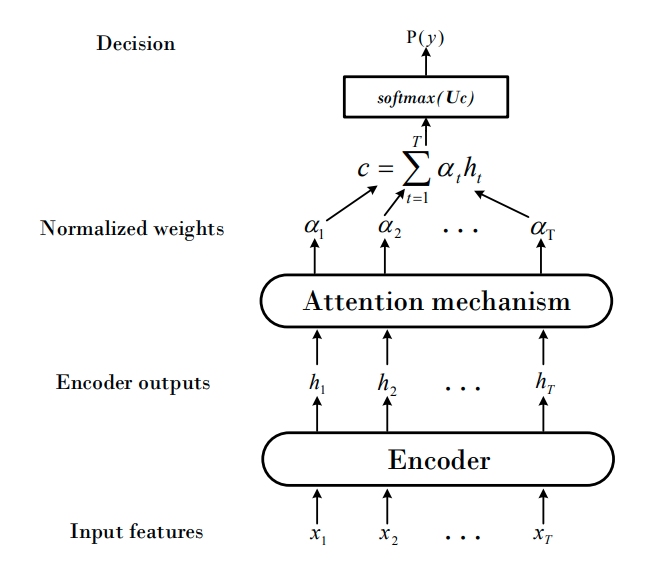
\includegraphics[width=0.5\textwidth]{figures/attention_arch.png}
                \caption{Attention-based end-to-end model for KWS.}
                \label{fig:attention_arch}
            \end{center}
        \end{figure}

        \begin{description}
            \item[Feature Extraction] The positive training sample has a frame length of $T = 1.9$ seconds which ensures the entire wake-up word is included. 
            Accordingly, in the attention models, the input window has set to 189 frames to cover the length of the wake-up word.
            Each audio frame was computed based on a 40-channel Mel-filterbank with 25ms windowing and 10ms frame shift. 
            Then the filterbank feature was converted to per-channel energy normalized (PCEN) [21] Mel-spectrograms.

            \item[Deep Neural Network] The overall architecture can be seen in figure \ref{fig:attention_arch}.
            The end-to-end system consists of an encoder and an attention mechanism. 
            The encoder transforms the input features into a high level representation using simple RNNs. 
            Then the attention mechanism weights the encoder features and generates a fixed-length vector.
            Two types of attention were investigated, average attention and soft attention
            \begin{itemize}
                \item \textbf{Average attention}: The \textit{Attention} model does not have trainable parameters and the $\alpha_{t}$ is set as the average of $T$:
                \begin{equation}
                    \alpha_{t} = \frac{1}{T}
                \end{equation}

                \item \textbf{Soft attention}: This attention method is borrowed from speaker verification \cite{abc}, the model learns the shared-parameter non-linear attention weights.
                First, model learns a scalar score $e_{t}$:
                \begin{equation}
                    e_{t} = v^{T}\tanh(Wh_{t} + b)
                \end{equation}

                Then the normalized weight $\alpha_{t}$ are computed using these scalar scores:
                \begin{equation}
                    \alpha_{t} = \frac{\exp(e_{t})}{\sum_{j=1}^{T}{\exp(e_{j})}}
                \end{equation}

            \end{itemize}

            Finally, by linear transformation and softmax function, the vector becomes a score used for keyword detection.
            To improve end-to-end approach, further encoder architectures were explored, including LSTM, GRU and CRNN.

            \item[Posterior Handling] Unlike some other approaches, the end-to-end system outputs a confidence score directly without post-processing.
            The attention-based system is triggered directly when the $p(y=1)$ exceeds a preset threshold.
        \end{description}

        Experiments on real-world wake-up data show that, with similar size of parameters, the attention models outperform Deep KWS by a large margin. 
        With encoder architecture, GRU is preferred over LSTM and the best performance is achieved by CRNN.

    \section{WaveNet-based small-footprint KWS} \label{sec:related_wavenet}

        Article \cite{wavenet} presented a end-to-end stateless temporal modeling which can take advantage of a large context while limiting computation and avoiding saturation issues.
        An architecture was explored based on a stack of dilated convolution layers, effectively operating on a broader scale than with standard convolutions while limiting model size. 
        Further improvement solution was to use with gated activations and residual skip-connections, inspired by the WaveNet style architecture explored previously for text-to-speech applications \cite{wavenet} and voice activity detection \cite{wavenet}, but never applied to KWS at the time the article was published.
        Moreover, ResNets differ from WaveNet models in that they do not leverage skip-connections and gating, and apply convolution kernels in the frequency domain, drastically increasing the computational cost.
        In addition, the long-term dependency the model can capture is exploited by implementing a custom ``end-of-keyword'' target labeling, increasing the accuracy of the model.

        \begin{description}

            \item[Feature Extraction] The acoustic features are 20-dimensional log-Mel filterbank energies (LFBEs), extracted from the input audio every 10ms over a window of 25ms.
            
            \item[Deep Neural Network] WaveNet was initially proposed in \cite{wavenet}, as a generative model for speech synthesis and other audio generation tasks.
            It consists in stacked causal convolution layers wrapped in a residual block with gated activation units as depicted in figure \ref{fig:wavenet_arch}.

            \begin{itemize}
                \item \textbf{Dilated convolution}: Standard convolutional networks cannot capture long temporal patterns with reasonably small models due to the increase in computational cost yielded by larger receptive fields. 
                Dilated convolutions skip some input values so that the convolution kernel is applied over a larger area than its own.
                The network therefore operates on a larger scale, without the downside of increasing the number of parameters. 
                The receptive field $r$ of a network made of stacked convolutions indeed reads:
                \begin{equation}
                    r = \sum_{i}{d_{i}(s_{i}-1)}
                \end{equation}

                where $d_i$ refers to the dilation rate ($d_i = 1$ for normal convolutions) and $s_i$ the filter size of the i-th layer. 

                \item \textbf{Gated activations and residual connections}: Gated activations units - a combination of $tanh$ and $sigmoid$ activations controlling the propagation of information to the next layer - prove to efficiently model audio signals.
                Residual learning strategies such as skip connections are also introduced to speed up convergence and address the issue of vanishing gradients posed by the training of models of higher depth. 
                Each layer yields two outputs: one is directly fed to the next layer as usual, but the second one skips it. 
                All skip-connections outputs are then summed into the final output of the network. 
                A large temporal dependency, can therefore be achieved by stacking multiple dilated convolution layers.
            \end{itemize}

            \begin{figure}
                \begin{center}
                    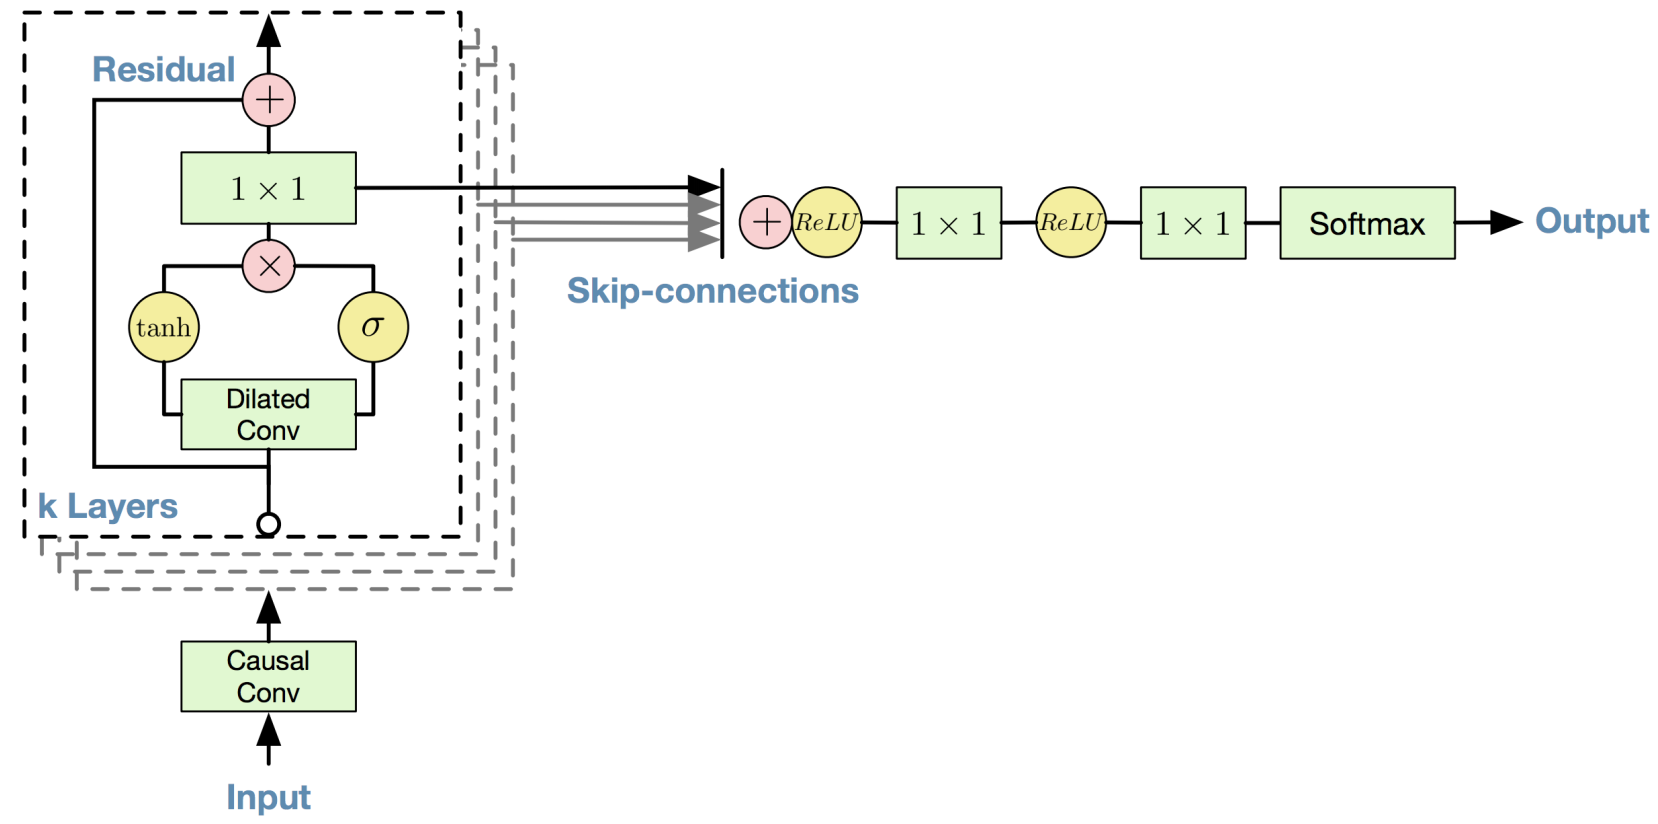
\includegraphics[width=0.7\textwidth]{figures/wavenet_arch.png}
                    \caption{WaveNet architecture.}
                    \label{fig:wavenet_arch}
                \end{center}
            \end{figure}

            \item[Posterior Handling] Like Deep KWS approaches, the end-to-end system computes smoothed posteriors by averaging the output of a sliding context window containing $w_{smooth}$ frames. However, the models do not require any postprocessing step besides smoothing, as opposed to others multi-class models.
            Indeed, the system triggers when the smoothed keyword posterior exceeds a pre-defined threshold.
        \end{description}


